\chapter{Pre-pattern recognition studies}\label{delta}
\textit{In the context of DAQ testing and performance analysis during Mu2e data-taking, 
where the data volume is expected to reach approximately 7 PBytes per year, optimizing 
memory usage and minimizing CPU consumption is crucial. The primary source of hits in the 
Mu2e tracker will be $\delta$-electrons. Therefore, it is essential to effectively flag these 
hits without compromising the efficiency of CE hit detection and track reconstruction. This 
Chapter presents a comparison between two algorithms designed for $\delta$-electron flagging.}

\section{$\delta$-electrons as source of background}

The primary source of hits in Mu2e is due to $\delta$-electrons, 
which mainly consist of Compton-scattered electrons, pair-production 
electrons and positrons, and delta rays, listed in decreasing 
order of prevalence. Compton-scattered electrons are produced 
when photons, generated by various processes, interact with the 
detector material. These photons primarily originate from 
neutron capture by atoms, which excites the nucleus and leads 
to photon emission during decay. Typically, these photons have 
energies of a few MeV. The neutrons are produced when muons are 
captured by atoms, resulting in unstable isotopes that decay by 
emitting neutrons. Pair-production electrons and positrons are 
generated during nuclear recoil processes, where pairs of electrons 
and positrons are created to conserve energy and momentum. Delta rays, 
or secondary ionization electrons, are generated when high-energy 
charged particles collide with the detector material.


\subsection{Compton scattering}
The Compton effect (Figure \ref{fig:compt}) refers to the 
scattering of a photon by a free or quasi-free electron. 
An electron is considered "quasi-free" when the energy of 
the incoming photon is significantly higher than the 
electron's binding energy ($E_\gamma \gg E_B$). The 
scattering process is termed Compton scattering if the 
electron is ejected from the atom, carrying away the 
recoil momentum. This effect is most prominent in an 
extended energy region around 1 MeV, with the region 
being much larger for low $Z$ materials compared to high $Z$ materials.

\begin{figure}[!h]
    \centering
    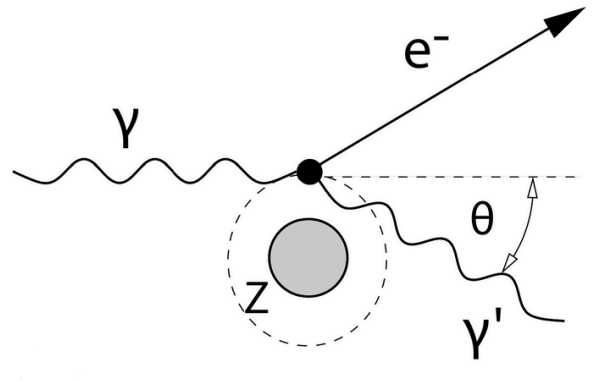
\includegraphics[width =0.4\textwidth]{figures/png/Screenshot_20240812_204345.png}
    \caption[The Compton effect.]{
    The Compton effect \cite{kola}.}
    \label{fig:compt}
\end{figure}

Since the photon scatters quasi-elastically off the electron, 
the energy and angle of the scattered photon are interdependent. 
To describe this relationship, we use the 4-momenta defined as 
follows: $k = (E_\gamma, \mathbf{k}c)$ and $p_e = (m_e c^2, 0)$ 
represent the 4-momenta of the photon and the electron (at rest) 
before scattering, and $k' = (E'_\gamma, \mathbf{k}'c)$ and 
$p'_e = (E'_e, \mathbf{p}'_e c)$ represent the 4-momenta 
after scattering. The angle between the scattered photon and 
the incident photon is denoted as $\theta_\gamma$, while the 
angle of the electron is denoted as $\theta_e$. By applying 
energy-momentum conservation:

\begin{equation}\label{compcons}
k + p_e = k' + p'_e
\end{equation}
\begin{equation}\label{compcons2}
(k - k')^2 = (p'_e - p_e)^2 \Rightarrow -k \cdot k' = m_e^2 c^4 - p'_e \cdot p_e
\end{equation}
\begin{equation}
\Rightarrow E_\gamma E'_\gamma (1 - \cos \theta_\gamma) = m_e c^2 \left(E'_e - m_e c^2\right) = m_e c^2 \left(E_\gamma - E'_\gamma \right)
\end{equation}

The right-hand side of the last equation uses the kinetic energy of the electron:

\begin{equation}
T = E'_e - m_e c^2 = E_\gamma - E'_\gamma
\end{equation}

which follows from the energy part of equation \ref{compcons}. 
The energy of the scattered photon as a function of the scattering 
angle is derived from equation \ref{compcons2}:

\begin{equation}\label{diffeq}
E'_\gamma = \frac{E_\gamma}{1 + \epsilon (1 - \cos \theta_\gamma)}
\end{equation}

where $\epsilon = \frac{E_\gamma}{m_e c^2}$.

The differential cross section per (free) electron, known as the 
Klein-Nishina formula, is calculated using methods from quantum electrodynamics:

\begin{equation}\label{kleinnishina}
\frac{d\sigma}{d\Omega} = \frac{r_e^2}{2} \frac{1 + \epsilon (1 - \cos \theta_\gamma)}{[1 + \epsilon (1 - \cos \theta_\gamma)]^2} \left(1 + \cos^2 \theta_\gamma + \frac{\epsilon^2 (1 - \cos \theta_\gamma)^2}{1 + \epsilon (1 - \cos \theta_\gamma)} \right)
\end{equation}

An electron bound in an atom can only be considered quasi-free 
if the photon's energy is significantly higher than the electron's 
binding energy. As the photon energy increases, more shell electrons 
become quasi-free, leading to the Compton cross section per atom 
approaching proportionality to $Z$, with individual electrons 
contributing incoherently:

\begin{equation}
\sigma_C^{\text{atom}} = Z\sigma_C
\end{equation}

where $\sigma_C$ is the Klein-Nishina cross section for a 
single free electron. The Compton cross section decreases at 
lower energies, where coherent scattering (Rayleigh scattering) 
off the entire atom (without ionizing the electron shell) becomes dominant.

By reformulating the Klein-Nishina formula, one can obtain the 
differential dependence of the Compton cross section on the 
kinetic energy of the recoil electron $T = E_\gamma - E'_\gamma$:

\begin{equation}
\frac{d\sigma}{dT} = \frac{\pi r_e^2}{m_e c^2 \epsilon^2} \left[2 + \frac{t^2}{\epsilon^2 (1 - t)^2} + \frac{t}{1 - t}\left(t - \frac{2}{\epsilon}\right)\right]
\end{equation}

where $t = T/E_\gamma$. Because the scattering process is 
elastic, there is a one-to-one relationship between the 
energy and angle $\theta_e$ of the electron:

\begin{equation}
\cos \theta_e = \frac{T(E_\gamma + m_e c^2)}{E_\gamma \sqrt{T^2 + 2m_ec^2 T}} = \frac{1 + \epsilon}{\sqrt{\epsilon^2 + 2\epsilon/t}}
\end{equation}

The maximum energy transfer to the electron is obtained 
from equation \ref{diffeq} for backward scattering of the 
photon ($\theta_\gamma = 180^\circ$), corresponding to 
forward scattering of the electron ($\theta_e = 0^\circ$). 
The electron's kinetic energy reaches its maximum value in 
this case, $T \rightarrow T_{\text{max}}$. In the measured 
energy spectrum, this leads to the so-called "Compton edge" at:

\begin{equation}
T_{\text{max}} = \frac{E_\gamma \cdot 2\epsilon}{1 + 2\epsilon}
\end{equation}

which lies slightly below the photopeak. The energy difference 
between the photopeak and the Compton edge $E'_\gamma(\theta = \pi)$ 
decreases with increasing $E_\gamma$ and approaches:

\begin{equation}
E'_\gamma(\theta = \pi) \approx \frac{m_e c^2}{2} \text{ for } E_\gamma \gg m_e c^2
\end{equation}

\subsection{Pair production}
In the Coulomb field of a charge, a photon can 
convert into an electron-positron pair (Figure 
\ref{fig:pprod})\footnote{Photon emission by an 
electron (bremsstrahlung) and pair production are closely 
related processes. By modifying the bremsstrahlung diagram-changing 
the outgoing photon to an incoming one and the incoming electron to 
an outgoing positron-one obtains the pair production 
diagram. The matrix elements of these processes are 
related, at least in the lowest order. Consequently, both 
processes are treated together in the foundational work by 
Bethe and Heitler, often referred to as the 'Bethe-Heitler processes'.}.

\begin{figure}[!h]
    \centering
    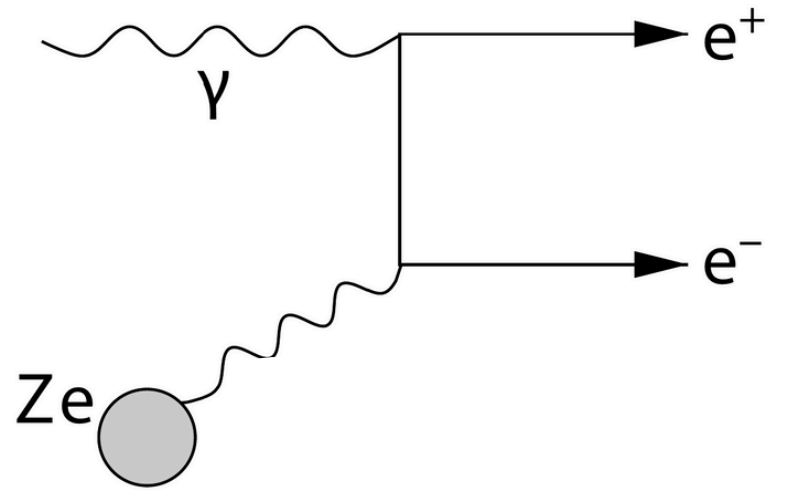
\includegraphics[width=0.4\textwidth]{figures/png/Screenshot_20240812_204755.png}
    \caption[The pair production.]{The pair production \cite{kola}.}
    \label{fig:pprod}
\end{figure}

The energy of the photon must exceed twice the electron 
mass plus the recoil energy transferred to the field-producing 
charge. For most elements, pair production predominantly 
occurs in the Coulomb field of the nucleus. For nuclei, 
the recoil energy is usually negligible, leading to a 
threshold energy for pair production of:
\begin{equation}
    E_{\gamma} \geq 2m_e c^2 + 2 \frac{m_e^2}{m_{\text{nucleus}}} c^2
\end{equation}

If the nuclear charge is not screened by atomic electrons 
(for low energies, the photon must come relatively close to 
the nucleus to make pair production probable, meaning it 
interacts with the "bare" nucleus),
\begin{equation}
    1 \ll \epsilon \ll \frac{1}{\alpha Z^{1/3}}
\end{equation}
the pair-production cross section is given by:

\begin{equation}
    \sigma_{\text{pair}} = 4 \alpha r_e^2 Z^2 \left(\frac{7}{9} \ln 2 \epsilon - \frac{109}{54}\right) \text{ cm}^2/\text{atom}
\end{equation}

However, for complete screening of the nuclear charge ($\epsilon \gg 1/\alpha Z^{1/3}$):
\begin{equation}\label{sigmapair}
    \sigma_{\text{pair}} = 4 \alpha r_e^2 Z^2 \left(\frac{7}{9} \ln \frac{183}{Z^{1/3}} - \frac{1}{54}\right) \text{ cm}^2/\text{atom}
\end{equation}

At high energies, pair production can occur even 
at relatively large impact parameters between the 
photon and the nucleus. In this case, the screening 
effect of atomic electrons must be considered. For 
large photon energies, the pair-production cross 
section approaches an energy-independent value as given by
 Equation \ref{sigmapair}. Ignoring the small term in the equation, 
 the asymptotic value of $1/54$ is expressed as:
\begin{equation}
    \sigma_{\text{pair}} \approx \frac{7}{9} \cdot 4 \alpha r_e^2 Z^2 \ln\left(\frac{183}{Z^{1/3}}\right) \approx \frac{7}{9} \cdot \frac{1}{X_0} \cdot \frac{A}{N_A \rho}
    \label{eq:paircross_radiationlength}
\end{equation}

The energy is uniformly distributed between the produced 
electrons and positrons at low and medium energies, but becomes 
slightly asymmetric at high energies.

The field of the nucleus is formed by the coherent sum of $Z$ 
nucleon charges, leading to the $Z^2$ dependence of the pair 
production cross section.

Even with large momentum transfers $\Delta p$ to the nucleus, 
the energy transfer $(\Delta p)^2/2M$ remains small due to the 
large nuclear mass $M$. After pair creation, the remaining 
energy is equally divided between the $e^+$ and the $e^-$.

\subsection{Delta rays}
High-energy $\delta$-rays, or $knock-on$ electrons, 
are produced when a projectile particle collides 
centrally with shell electrons, resulting in 
significant energy transfers. These electrons 
gain high kinetic energy and can be described 
through elastic collisions with quasi-free electrons. 
By considering the energy-momentum conservation relation 
and using the Lorentz factors $\gamma$ and $\beta$, the 
relationship between the kinetic energy $T$ of the 
$\delta$-ray and the emission angle $\theta$ can be derived as:

\begin{equation}
\cos \theta = \frac{T(\gamma + m_e / M)}{\gamma \beta \sqrt{T^2 + 2T m_e c^2}}
\end{equation}

\begin{equation}
T(\theta) = \frac{2 m_e c^2 \beta^2 \gamma^2 \cos^2 \theta}{\gamma^2(1 - \beta^2 \cos^2 \theta) + 2 \gamma m_e / M + m_e^2 / M^2}
\end{equation}

The maximum energy transfer $T_{\text{max}}$ occurs at $\theta = 0^\circ$, 
while the minimum energy, $T_{\text{min}}$, occurs at $\theta = 90^\circ$. 
At highly relativistic energies ($\gamma \gg 1$ and $\theta \gg 1/\gamma$), 
the energy-angle relationship becomes independent of the incoming particle's properties.

The rate of $\delta$-rays per energy interval $dT$ and path length $dx$ is given by:

\begin{equation}
\frac{d^2 N}{dx \, dT} = n_e \frac{d\sigma}{dT}
\end{equation}

which, when combined with the electron density and the differential cross section, becomes:

\begin{equation}
\frac{d^2 N}{dx \, dT} = \frac{1}{2} z^2 \frac{Z}{A} K \rho \frac{1}{\beta^2} \frac{F(T)}{T^2}
\end{equation}

Here, $K$ is the constant from the Bethe-Bloch formula, 
and $F(T)$ is a function accounting for spin dependence. 
Integration over $T$ and $x$ provides the number of $\delta$-rays in a medium of thickness $\Delta x$:

\begin{equation}
N = \frac{1}{2} z^2 \frac{Z}{A} K \rho \Delta x \frac{1}{\beta^2} \left(\frac{1}{T_{\text{min}}} - \frac{1}{T_{\text{max}}}\right) \approx 0.077 \frac{\text{MeV cm}^2}{\text{g}} z^2 \rho \Delta x \frac{1}{T_{\text{min}}}
\end{equation}

The emission angle dependence is given by:

\begin{equation}
\frac{dT}{d \cos \theta} = 4 m_e c^2 \frac{\cos \theta}{\sin^4 \theta}
\end{equation}

Substituting this into the rate equation yields:

\begin{equation}
\frac{d^2 N}{dx \, d \cos \theta} = \frac{1}{2} z^2 \frac{Z}{A} K \rho \frac{1}{\cos^3 \theta} \frac{1}{m_e c^2} \approx 0.15 \frac{\text{cm}^2}{\text{g}} z^2 \rho \frac{1}{\cos^3 \theta}
\end{equation}

This expression diverges as $\theta$ approaches $90^\circ$, 
where $T$ approaches zero, indicating a limitation in the 
assumption of a free electron. The resulting distributions 
suggest that $\delta$-rays emitted at small angles can 
significantly affect the spatial resolution in detectors, 
particularly through ionization clusters that broaden the 
track of the mother particle.



\section{Monte Carlo samples}\label{datasample}
For our studies, we used three distinct Monte Carlo data samples: two were 
related to CEs combined with two different proton pulse intensity, while the third was 
dedicated to antiproton annihilation events. The production of particles within 
the PT and their tracking from the PS to the DS is managed using the Mu2e Offline software 
(Appendix \ref{mu2eana}). The simulation of particle interactions is based on 
GEANT4, while the event processing is handled by the art framework and data 
management is governed by the SAM system.

The Mu2e simulation employs a technique known as multi-stage simulation 
to generate and simulate events efficiently. This method involves generating 
events, partially simulating them, and then pausing the process to save the 
data generated thus far. Later stages resume the simulation from the saved 
state. This approach optimizes both the time required for event generation 
and the usage of computing resources. The simulation is divided into seven 
stages, S0 through S6, which will be briefly discussed in the context of our specific needs:

\begin{itemize}
    \item \textbf{Stage 0}: primary beam protons are generated and propagated 
    inside the PT. When an inelastic interaction occurs at the target, the vertex 
    position is recorded, and the propagation is halted. The probability of 
    inelastic interactions is determined by the total inelastic cross-section 
    ($\sigma_{\text{tot.inelastic}}$) of protons on tungsten (W), which follows the 
    empirical cross section $\sigma_{\text{tot.inelastic}}(\text{W}) = (1710 \pm 30) \ \text{mb}$.
    The probability that a proton from the beam induces an inelastic interaction with the tungsten target is computed using a Monte Carlo approach 
    ($    \frac{N_{\text{inelastic}}}{N_{\text{POT}}} = 0.792$). Regarding the $\bar{p}$ 
    data sample, the number of antiprotons produced per proton on target (POT) at the production target is given by:
    $$
    N_{\bar{p}_{\text{POT}}} = \frac{\sigma_p}{\sigma_{\text{tot.inelastic}}} \times N_{\text{inelastic}} = \frac{0.5 \times 0.2824 \, \text{mb}}{1710} \times 0.792 = 6.5 \times 10^{-5}.
    $$
    Antiprotons are generated with a flat momentum distribution between 0 and 5 GeV/c and 
    are assumed to have isotropic directions;
    
    \item \textbf{Stage 1}: events are propagated through the TS and PS. 
    Only those particles that reach a virtual detector (VD) in front 
    of the TS entrance are saved as input for the next stage;

    \item \textbf{Stage 2}: in this stage, $\pi^-$, $\mu^-$, and $\bar{p}$ 
    particles are stored and tracked. To enhance statistics, a resample factor 
    is applied here: each $\bar{p}$ from S1 is traced multiple times, creating 
    independent events due to statistical fluctuations in energy losses within 
    the absorbers. A resample factor of $10^5$ keeps oversampling under control;

    \item \textbf{Stage 3}: particle transportation from the COL3u exit to the TS5 entrance;

    \item \textbf{Stage 4}: particle transportation from TS5 to the ST, 
    where the positions of stopped pions and muons are stored;

    \item \textbf{Stage 5}: to optimize simulation efficiency, $3 \cdot 10^7$ 
    stationary pions and antiprotons are generated at rest at the stopping 
    target, using the recorded time and position of the stops. These particles 
    are then propagated to the detectors. For the CE dataset, a fraction of muons 
    are assumed to decay into conversion electrons. For the $\bar{p}$ dataset, 
    antiproton annihilation at rest in the ST is simulated based on the positions 
    and times of the stopped antiprotons. Background electrons from annihilation 
    result from decays such as $\pi^0 \to \gamma \gamma$, followed by photon 
    conversions, and $\pi^- \to \mu^- \nu$, followed by $\mu^-$ decays. During 
    this stage, the raw simulated data are digitized into simple C++ classes or 
    structs, mimicking the detector's raw data;

    \item \textbf{Stage 6}: Finally, reconstruction from detector hits is performed.
\end{itemize}

Regarding CPU time, Stages 0 and 1 are the most time-consuming. 
Stage 2 can also be demanding when a high resampling factor is used, 
while the later stages are significantly faster by an order of magnitude.

A typical Mu2e event includes multiple hits from particles produced 
by muon captures in the ST, as well as particles entering the DS from 
the TS. These hits are called pileup hits, which make 
up the majority of the detector's hits. The pileup level 
depends on the proton pulse intensity. The Mu2e pileup 
simulation assumes that the pulse intensity varies on a 
time scale much longer than 2 $\mu$s, meaning all proton 
pulses around the simulated one share the same intensity. 
Under this assumption, a transformation is applied to hits 
with time $T_i > 1695$ ns outside the microbunch limits, 
assigning them a new time $t_i = \frac{T_i}{1695}$ ns, 
effectively accounting for late hits that would otherwise 
be attributed to later microbunches. 

For low-intensity (1BB) mode, with a mean intensity of 
$1.6 \times 10^7$ protons/pulse, approximately 25,000 
muons stop in the ST per pulse. In the high-intensity 
(2BB) mode, this number is about 2.5 times higher (Section \ref{pulsedprotonbeam}).

The datasets used for conversion electron plus pileup 
analysis will be referred to as $CELE1BB$ and $CELE2BB$ 
for 1BB and 2BB pileup, respectively. The dataset for 
antiproton analysis without pileup will be referred to as $PBAR0BB$.
For datasets with pileup, 
the pileup hits are explicitly added to the hits from 
the signal process. In this case, however, no pileup hits 
are added, meaning the data represents pure signal. 
\section{$\delta$-electrons producing hits in the Mu2e tracker}

In the Mu2e experiment, low-energy electrons and positrons, referred to as $\delta$-electrons, 
with a momentum below 20 MeV/c, constitute the majority of the tracker hits. Managing these 
hits is crucial for optimizing memory efficiency and CPU consumption. From a physics point 
of view, there are different reasons why it is important to identify those hits:
\begin{itemize}
    \item the signal we want to observe is the CE. Flagging even a small fraction of 
    potential CE hits is extremely dangerous, as it could result in the failure to 
    reconstruct the corresponding tracks.
    As shown in the histogram in Figure \ref{fig:momhits}, the simulated CE hits make up 
    just 1\% of the total hits in the tracker;
    \item flagging protons would assist the STM in counting the muon stopping rate. 
    It is possible to estimate the number of muons captured in the stopping target 
    by counting the number of protons produced during nuclear muon capture, 
    which is one of the possible processes a stopped muon can undergo (61\%);
    \item misidentifying muons and pions as protons or $\delta$-electrons could lead to a 
    incorrect estimate of the background events. This is particularly significant for the antiproton background.
    $p\bar{p}$ annihilation at rest in the ST can produce events with more than one track, 
    each with a momentum around 100-200 MeV/c. For $p\bar{p}$ annihilation events 
    in the ST, the rate of multi-track events is about 500 times higher 
    than the rate of events with a single signal-like electron. 
    For $10^4$ $p\bar{p}$ annihilation events generated, about 3.7\% of 
    the events contained two reconstructable particle tracks. Therefore, 
    the identification and reconstruction of multi-track events could be 
    used to constrain the $\bar{p}$ background. Thus, it is crucial
     not to flag muons or pions, as the fraction of multi-track events is very low.
\end{itemize}
Figure \ref{fig:momhits} shows the true momentum distribution of 
hits that make at least one hit in the tracker in the case of a 
dataset containing at least one CE per event. Each momentum bin is filled with 
the number of hits corresponding to a specific Monte Carlo particle. 
The data sample description used to perform this distribution 
is presented in Section \ref{datasample}.
The distribution reveals that the majority of hits originate from 
low-energy electrons and positrons (orange), constituting approximately 
75\% of the total number of hits. This histogram corresponds to 
the 1BB pileup scenario. 
There is an asymmetry between the number of hits below 20 MeV/c 
produced by electrons and positrons: electrons account for 
71\% of all $\delta$-electron hits in the tracker, while positrons 
contribute only 4\%. This discrepancy arises because only electrons 
undergo Compton scattering, which is the primary source of hits at 
energies around 1 MeV. This difference will be crucial in 
the following sections when discussing the $\delta$ flagging efficiency.

As evident from the histogram, 14\% of the total hits are due to protons, 
which are produced by nuclear processes. 
In particular, the first peak in protons momentum distribution arises from 
inelastic neutron scattering and while larger momentum values correspond muon capture at rest.
Their kinetic energy ranges from about 5 to 20 MeV, resulting in low $\beta \gamma$ values, 
making them heavily ionizing particles. The deposited energy will be 
one of the variables used to discriminate protons. 

It is important to note that the bump around 50 MeV/c in 
the positron distribution should not be present. According 
to the Monte Carlo truth, this is due to muon Decay-In-Flight, 
and we expect $N(\mu^+ \rightarrow e^+ )/N(\mu^- \rightarrow e^- )$ to be about $10^{-3}$ 
for muons entering the DS. The Decay-In-Orbit on the IPA 
(Section \ref{detectorsolenoid}) should also be around 
$10^{-3}$ compared to the DIF of negative muons. 
The simulation of $\mu^+$ may contain some errors, 
which we have reported to the simulation specialists. 
However, this issue is not problematic for the analysis 
of low-momentum electrons and positrons, as the momentum ranges are different.

\begin{figure}[!h]
        \centering
        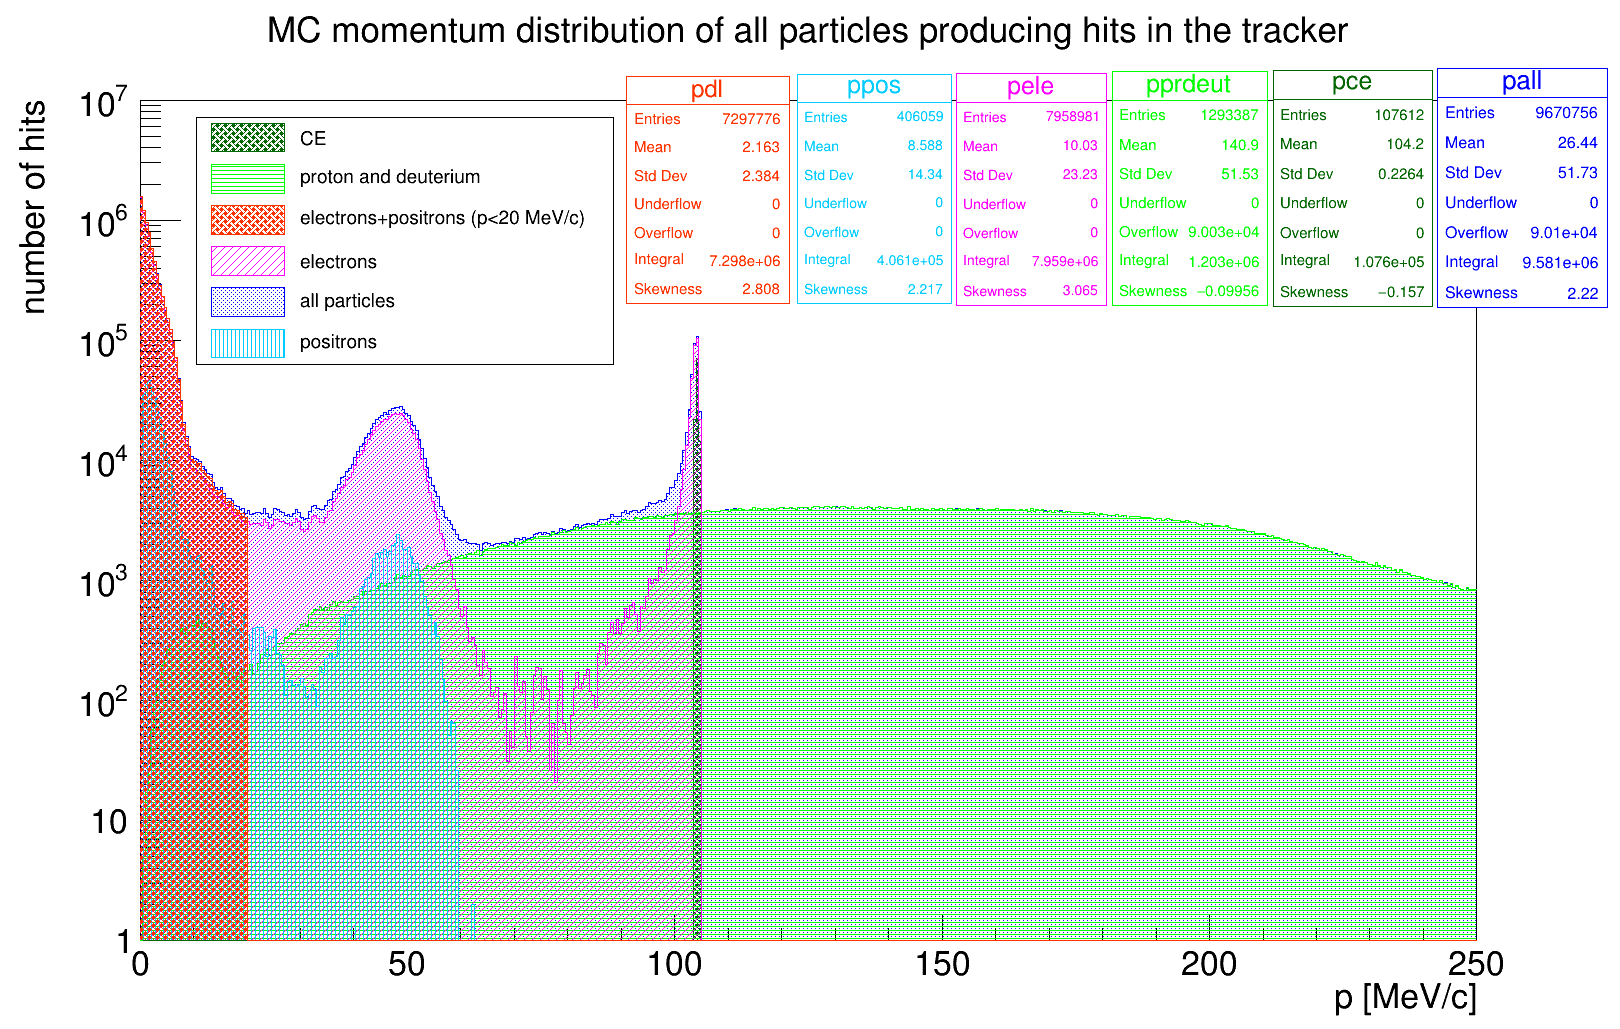
\includegraphics[width =0.95\textwidth]{figures/png/Screenshot_20240812_152905.png}
    \caption[Monte Carlo momentum distribution of particles producing hits in the Mu2e tracker (conversion electron dataset and pileup).]{
       The Monte Carlo momentum distribution of particles producing at 
       least one hit in the Mu2e tracker (conversion electron dataset and pileup). The distribution
       corresponds to 1BB pile-up. The momentum distribution 
       of all particles making hits is depicted in dark blue, with electrons 
       shown in pink, positrons in light blue, $\delta$s in orange, protons and deuterons in 
       light green, and CEs in dark green. }
       \label{fig:momhits}
\end{figure}


Figure \ref{fig:pbar} shows the true momentum distribution of 
particles produced in the $p\bar{p}$ annihilation at the ST. 
The data sample description used to perform this distribution 
is presented in Section \ref{datasample}.
Each momentum bin contains the number of hits corresponding 
to a specific Monte Carlo particle. The dataset used to generate 
this histogram has no pileup (0BB). 
The particles produced in the $p\bar{p}$ annihilation 
are mostly pions, muons, and a few electrons. 
It can be observed that the momentum distribution 
peaks in the 100-200 MeV/c range. Photons are also 
produced, and they can undergo Compton scattering and 
pair production, which explains the presence of a 
$\delta$-electron peak that is about $\sim$100 
times lower than the peak in Figure \ref{fig:momhits}.

\begin{figure}[!h]
    \centering
    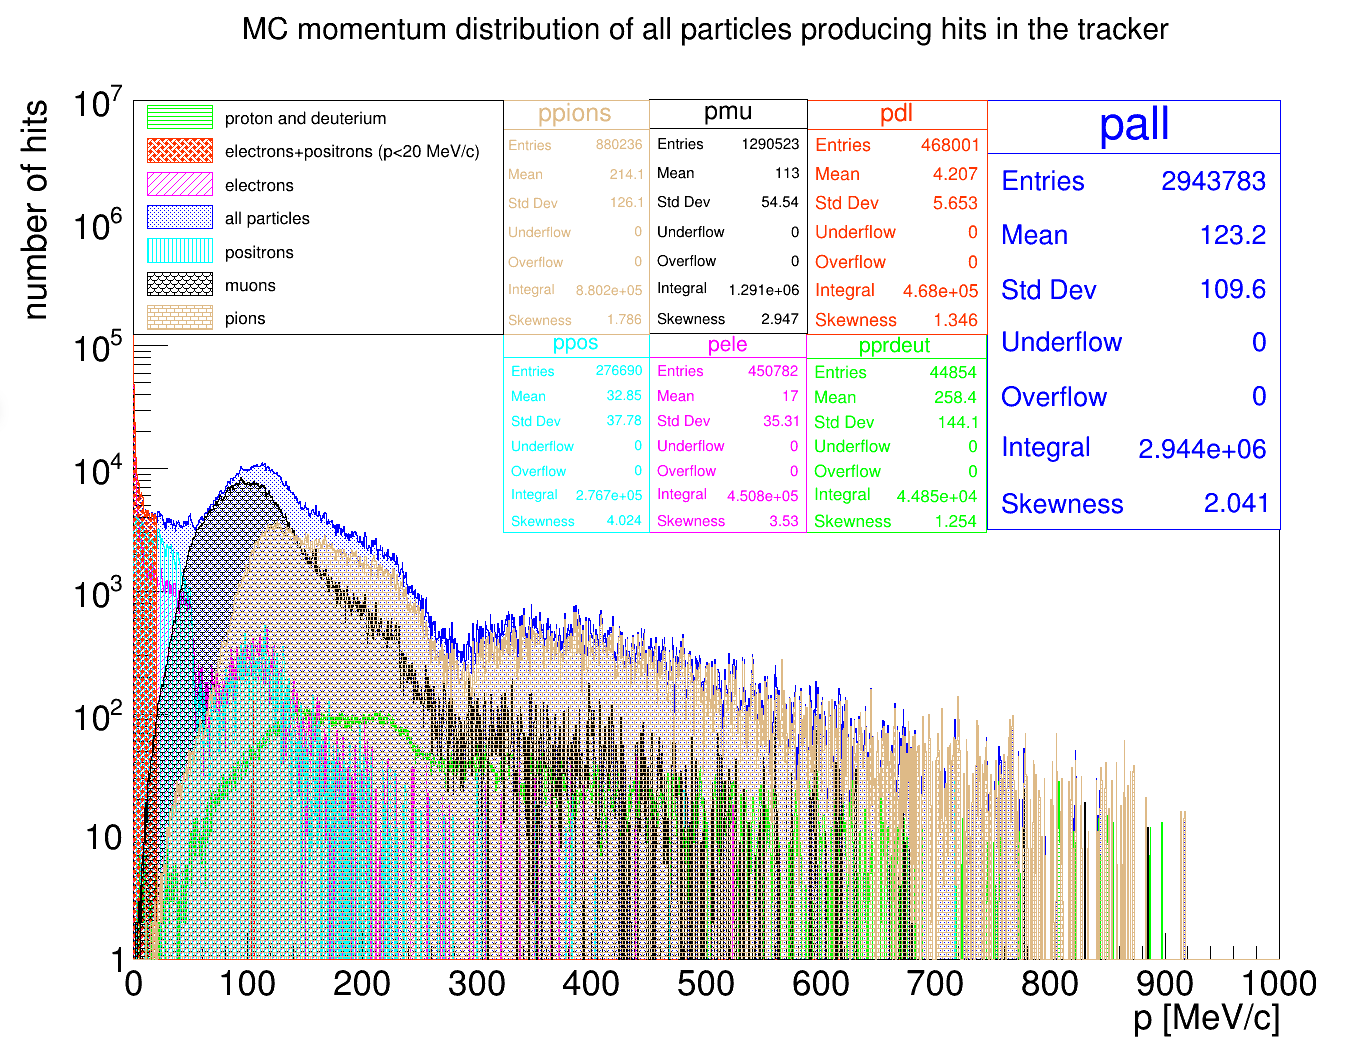
\includegraphics[width =0.9\textwidth]{figures/png/Screenshot_20240815_124710.png}
\caption[Monte Carlo momentum distribution of particles producing hits in the Mu2e tracker ($\bar{p}$ dataset and no pileup).]{
   The Monte Carlo momentum distribution of particles producing at 
   least one hit in the Mu2e tracker ($\bar{p}$ dataset and no pileup). 
   The momentum distribution 
   of all particles making hits is depicted in dark blue, with electrons 
   shown in pink, positrons in light blue, $\delta$s in orange, protons and deuterons in green, pions in light brown and muons 
   in black. }
   \label{fig:pbar}
\end{figure}

As shown in Figure \ref{fig:momhits}, the majority of the recorded hits 
originate from $\delta$-electrons, with protons being the second most 
common source. Figure \ref{fig:afbef} presents an example of comparison of an 
event before and after the background hits have been flagged. 
Flagging these hits is crucial for several reasons: it prevents unnecessary 
data from being sent to the pattern recognition algorithms, thereby conserving 
CPU resources and reducing processing time. Moreover, it is important to avoid 
storing these hits on tape, as doing so would lead to inefficiencies in data storage.

\begin{figure}[!h]
    \begin{subfigure}[b]{0.4\linewidth}
        \centering
        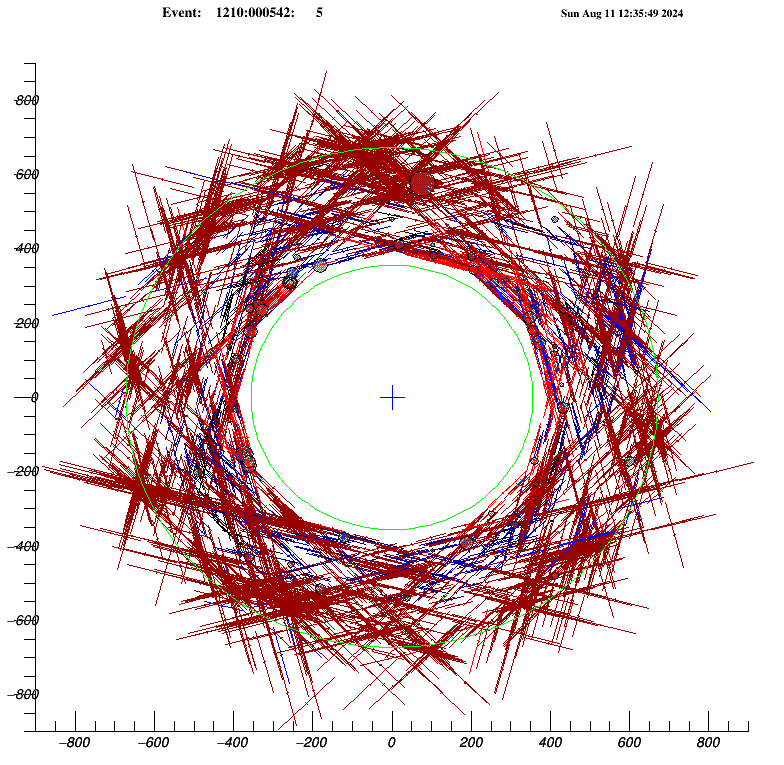
\includegraphics[scale = 0.3]{figures/png/Screenshot_20240811_123612.png}
        \subcaption{Before.}
        \label{fig:bef}
    \end{subfigure}
    \begin{subfigure}[b]{0.7\linewidth}
        \centering
        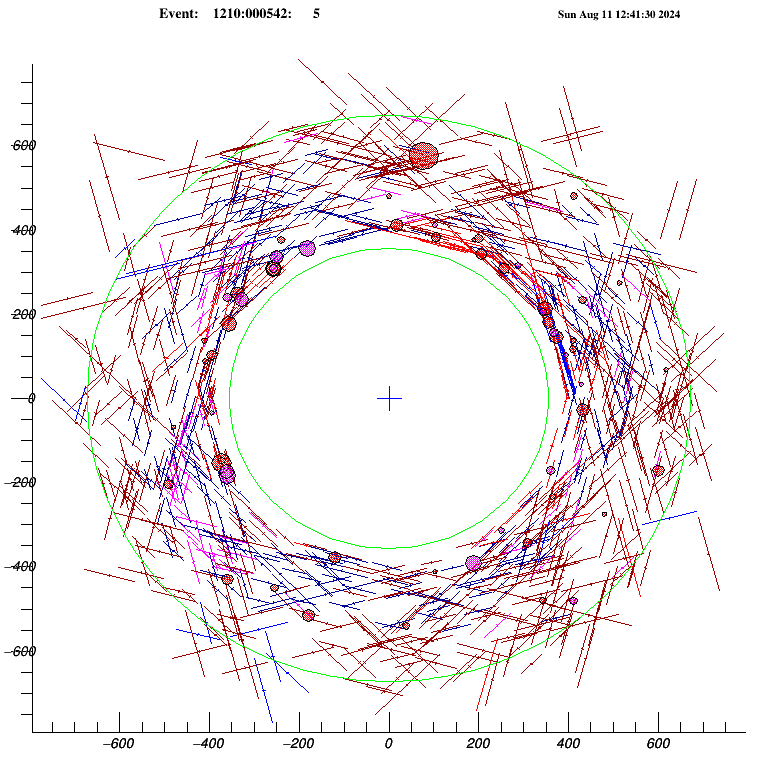
\includegraphics[scale = 0.3]{figures/png/Screenshot_20240811_124245.png}
        \subcaption{After.}
        \label{fig:af}
    \end{subfigure}
    \caption{Before and After background hits flagging. The transverse $x-y$ views of a CE 
    event with 2BB pile-up (Section \ref{pulsedprotonbeam}). The segments are the $hit$ tracker straws. The hits marked in
    red are from electrons and the ones in blue are from positrons.}
    \label{fig:afbef} 
\end{figure}






\section{Mu2e $\delta$-electrons rejection algorithms}
The Mu2e Offline software tool is illustrated in 
Appendix \ref{mu2eana}, and the reconstruction 
process is described in Appendix \ref{eventreco}. 

The flagging of $\delta$-electrons is a step in the 
Mu2e reconstruction process that occurs before time clustering and pattern recognition.

In Mu2e Offline, there are two types of flagging algorithms:
\begin{itemize}
    \item $FlagBkgHits$, described in Section \ref{flagbkghits};
    \item $DeltaFinder$, described in Section \ref{deltafinder}.
\end{itemize}

\subsection{The $FlagBkgHits$ Algorithm}\label{flagbkghits}
The detailed description of multivariate analysis (MVA) and the 
process of MVA training are beyond the scope of this work. 
Nevertheless, since this technique is one of the options 
developed for background flagging, I will briefly outline 
the fundamental principles involved.

When searching for patterns in a multivariable space, 
a common procedure involves defining a set of statistical 
models that analyze the measured variables and estimate 
the probability that these are consistent with the 
sought pattern. Once the variables are selected, 
the MVA is trained to recognize patterns by 
evaluating examples known to the trainer, 
allowing for feedback to refine the 
pattern identification process.

The first selection concerns the mean energy deposited in  
the $ComboHit$s used to create a $StereoHit$ and excludes 
those with a deposited energy above 5 keV. 
The algorithm then classify as protons all hits with a deposited energy above 4.5 keV.
Other selections concern the timing, position, and spread of the $ComboHit$ 
in the $x$-$y$ plane. The maximum cluster timing 
and diameter are 20 ns and 5 mm, respectively.

Since $\delta$-electrons tend to form small, dense 
clusters of hits on $x$-$y$ plane, an algorithm based on a clustering 
approach was developed: concentrated clusters in the 
$x$-$y$ plane are sought using a clustering algorithm, 
as $\delta$-electrons are highly likely to reside 
in such clusters. The $FlagBkgHits$ algorithm employs 
a hit-level MVA to ensure that hits within a 
$\delta$-dominant cluster truly belong there, 
and a cluster-level MVA to differentiate 
$\delta$-dominant clusters from those 
predominantly containing conversion electrons. 
This was trained in a supervised mode, using CE and $\delta$-electrons hits from 
Monte Carlo data sample.

The current resolution of straw drift tube 
position measurements is limited to a few cm. 
However, an improved position measurement can be 
achieved by leveraging the multiple straw layers that 
significantly overlap in the transverse plane. 
By obtaining two hit measurements from a pair of 
intersecting straws and ensuring they fall within 
a time window on the order of the maximum drift time, 
one can deduce that these hits were produced by the 
same particle and occurred at the intersection of the 
two straws in the projected plane. This method, 
involving two-dimensional information from the two 
straws, is referred to as the stereo information method.

The clustering process uses the $x$ and $y$ coordinates 
of the selected hits. A random hit is chosen to define 
the initial cluster, after which the following iterative 
steps are applied. The centroid of each cluster is 
computed, and hits whose distances from a cluster 
centroid fall within a specified inner threshold 
and time window are added to that cluster. Hits 
with distances from all existing clusters greater 
than an outer threshold are used to seed new 
clusters, while hits that fall between the two 
thresholds remain unassigned. This process 
generates a new set of clusters, preparing the 
system for the next iteration. During each 
iteration, every hit is reconsidered as a 
potential new point in a cluster, including 
those already assigned. The clustering process 
continues until convergence is achieved, i.e., 
when an iteration no longer results in any changes.


\subsection{$DeltaFinder$ Algorithm}\label{deltafinder}

$DeltaFinder$ is an algorithm designed to identify $\delta$-electron 
hit patterns rather than CE hits. This algorithm relies on the 
fact that $\delta$-electrons typically form a straight line in 
the $r$-$z$ plane (cyan lines in Figure \ref{fig:yzviewdelta}) 
and appear as a spot with a diameter of less than 3 cm in the 
$x$-$y$ plane within the Mu2e magnetic field. In contrast, 
CE hits create entirely different patterns, appearing as oblique lines in 
the $r$-$z$ plane due to their helical trajectories (red lines in Figure \ref{fig:yzviewdelta}). 
In the process, all hits associated with detected objects are treated as $\delta$-electron hits.
\begin{figure}[!h]
    \centering
    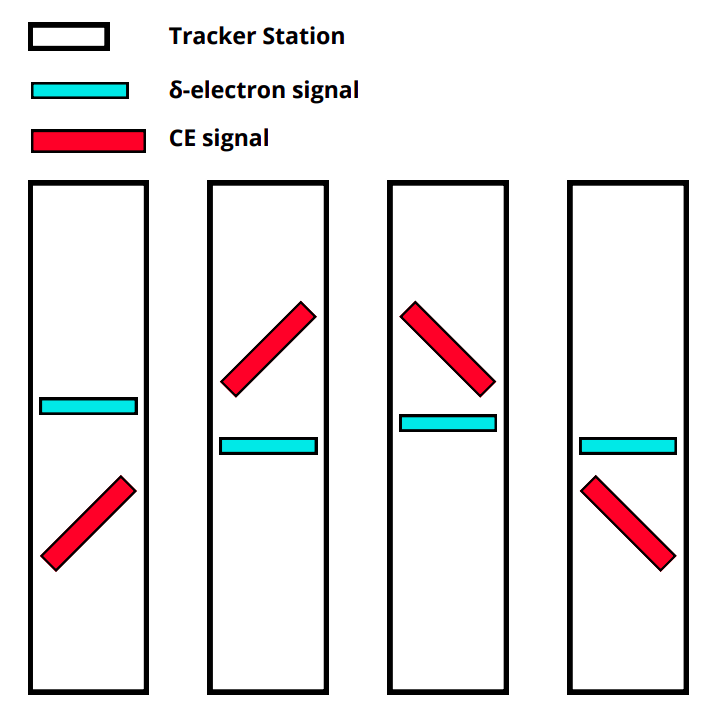
\includegraphics[width =0.6\textwidth]{figures/png/Screenshot_20240811_123048.png}
    \caption[$\delta$-electrons and CE patterns in $r-z$ plane.]{
        $\delta$-electrons and CE patterns in the $r-z$ plane. 
        The white squares represent some of the tracker stations. 
        The cyan straight lines represent the $\delta$-electron 
        patterns in the $r-z$ plane, while the red lines a CE signal in the same plane.
        }
    \label{fig:yzviewdelta}
\end{figure}
\subsubsection{Step 1: Identifying $\delta$-Electron Segments}
$DeltaFinder$ first seeks to identify $\delta$-electron track 
segments within each station individually. These segments, 
parallel to the beam axis, are called $seeds$. Since hits 
from the same electron should be close in both time and space, 
and $\delta$-electrons may hit multiple straws within the 
same panel, the algorithm clusters these straw hits in 
space-time, applying various cleanup cuts to ensure the 
selected patterns resemble $\delta$-electron hits. 
The maximum allowed time difference between two hits within 
a station to form a $seed$ is set to 40 ns.

These cleanups based on the $x$-$y$ coordinates are performed 
by computing a $\chi^2$. The $seed$ is reconstructed using 
two, three, or four $ComboHit$s. In each case, the 
intersections between two straws are determined, 
and the $x$-$y$ coordinates of the $seed$ are given 
by the center of gravity of these intersections. 
In the case of only two hits, the center of gravity 
corresponds to the stereo hit. Explicit stereo hit 
reconstruction is not used for all hits.

The algorithm extends the $seed$s by requiring 
hits to be sufficiently close to the intersection 
point in time and space, performing multiple checks 
to avoid over-efficiency in hit flagging. For each $seed$, 
the mean deposited energy is calculated from the energy 
deposited in all $ComboHit$s. Based on the mean 
deposited energy of a $seed$ in a station, hits with 
energy above 5 keV are considered proton hits. 
This selection optimizes data processing by 
reducing the total number of hits that need to be analyzed.

\begin{figure}[!h]
    \centering
    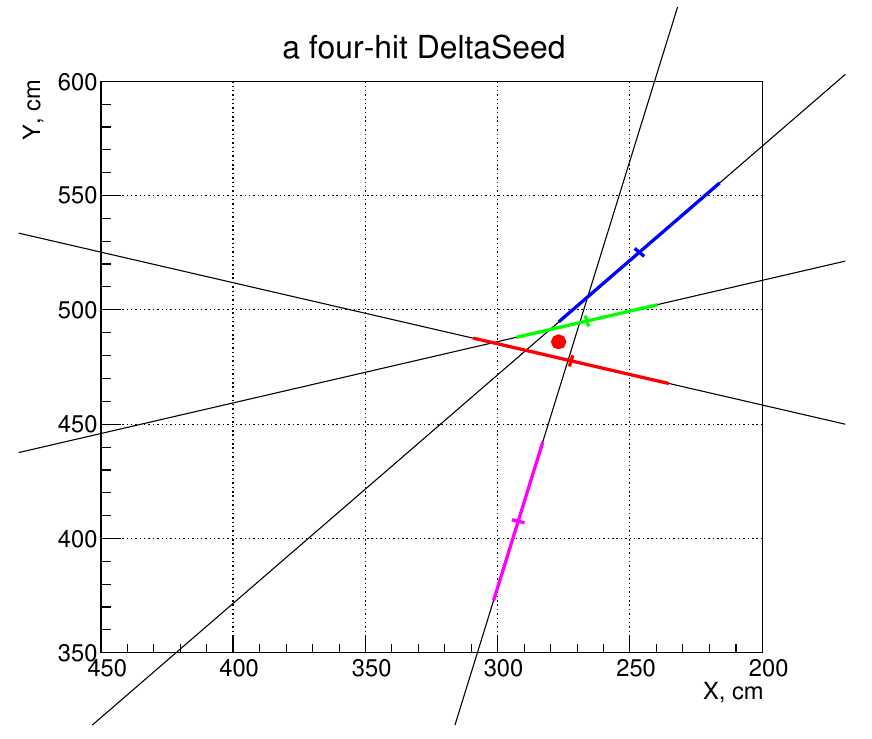
\includegraphics[width =0.6\textwidth]{figures/png/Screenshot_20240811_115854.png}
    \caption[A $\delta$ candidate $seed$.]{A $\delta$ candidate $seed$. The four coloured segments are the tracker straws that were
    hit in one station.}
    \label{fig:deltaseeds}
\end{figure}

It is necessary to do a clarification. 
Figure \ref{fig:energydeposited} shows the 
distribution of the simulated deposited energy 
in the tracker for $\delta$ electrons, CEs, and 
protons in the case of a 1BB pileup. 

To optimize data processing, a hit energy 
threshold could be applied to the $DeltaFinder$ 
to reduce the total number of hits that need to be analyzed, 
thereby speeding up the process. Moreover, only about 
4\% of CE hits have energies above 3.5 keV 
(and 1\% above 5 keV), so the loss of CE 
hits would be minimal, resulting in a faster overall algorithm. 

However, implementing such an energy cutoff has 
significant implications for the algorithm's performance. 
Starting with fewer hits, especially in stereo intersections, 
decreases the likelihood of identifying the correct $seed$. 
Additionally, a higher energy cutoff increases 
the probability of false positives, as the algorithm 
aims to count protons too.

\begin{figure}[!h]
    \centering
    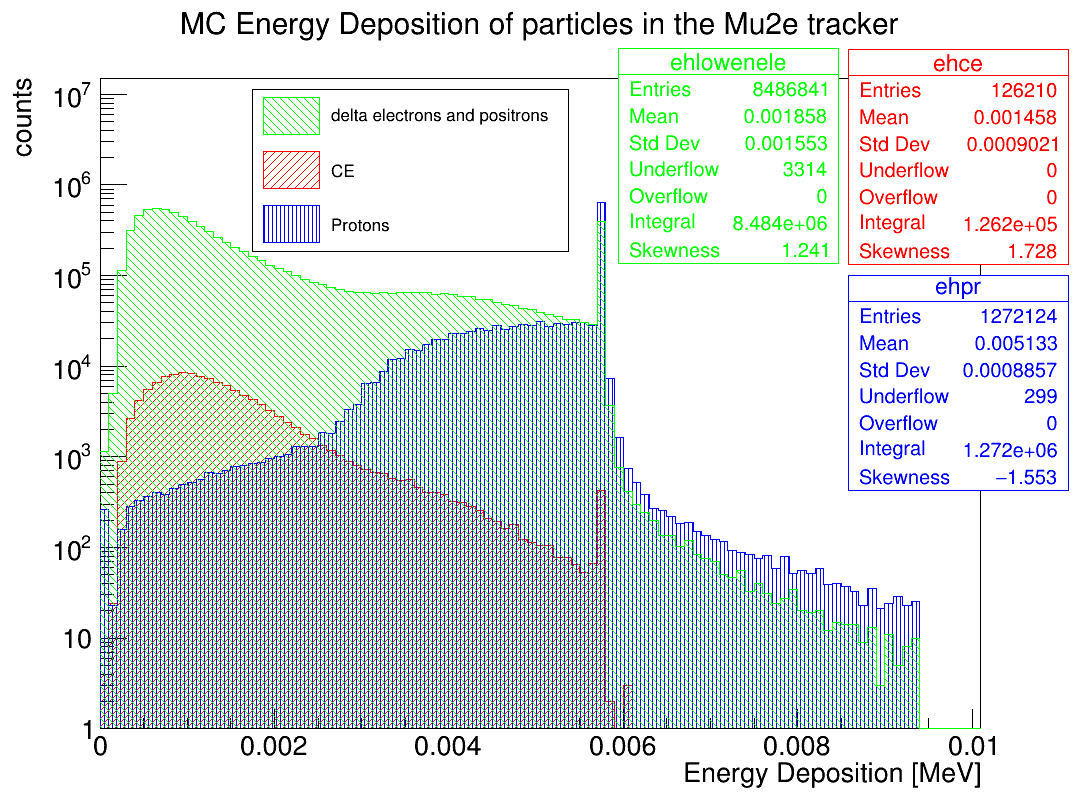
\includegraphics[width =0.8\textwidth]{figures/png/Screenshot_20240729_151910.png}
\caption[Monte Carlo deposited energy distribution in the Mu2e tracker.]{
   The Monte Carlo deposited energy distribution in the Mu2e tracker. The distribution
   corresponds to 1BB pile-up (Section \ref{pulsedprotonbeam}). The red distribution refers to 
   conversion electrons, while the green and the blue one to $\delta$-electrons and protons respectively. 
   The peaks and tails correspond to the saturation of the waveforms.

}
   \label{fig:energydeposited}
\end{figure}
\subsubsection{Step 2: Connecting $seed$s}
After the selection based on mean deposited energy, 
$DeltaFinder$ attempts to connect segments that 
are close in both the $x$-$y$ plane and time 
across different stations to form $\delta$-electron 
candidates. A valid candidate must have at 
least two segments and a minimum of five straw hits. 
Reconstructed segments from a 100 MeV electron 
typically remain unconnected due to their separation in the $x$-$y$ plane. 

$DeltaFinder$ links $\delta$-electron $seed$s 
across stations, attempting to associate new $seed$s 
with existing $\delta$ candidates. If no match is 
found, a new candidate is created. Good $\delta$ 
candidates are marked, and their hits are 
flagged to prevent their inclusion in proton candidate searches.

\subsubsection{Step 3: Identifying Proton Candidates}
Finally, $DeltaFinder$ identifies proton candidates 
using the remaining $seed$s, which are more likely 
to have deposited energy above 3 keV. First, it checks 
if a $seed$ is consistent in time with any existing 
proton candidates. If no consistency is found, 
the hits of the $seed$ are added to a new proton candidate.


\section{Analysis of the performance and comparison}
The analysis is carried out on two levels of 
comparison, each addressing different aspects of the algorithms under evaluation:

\begin{itemize}
    \item \textbf{Hit-level comparison}: This phase focuses 
    on evaluating how accurately individual hits are 
    flagged, providing the most direct method for 
    assessing and comparing the performance of the two 
    algorithms. This stage allows for an unbiased 
    comparison without the influence of subsequent 
    reconstruction stages. It also includes a direct evaluation of proton counting;
    
    \item \textbf{Track-level comparison}: This phase examines 
    the algorithms' impact on the later stages of 
    event reconstruction. It highlights how effectively 
    each algorithm contributes to the accurate reconstruction 
    of tracks. The main figure of merit at this stage is the 
    reconstruction of CE tracks, as well as muons and pions, which are crucial 
    for estimating the background level.
\end{itemize}

\subsection{Hit-level comparison}
Before starting with the hit-level comparison of the two algorithms, during the analysis, 
we first observed an over-efficiency in the proton hit flagging by $DeltaFinder$. 
This primarily impacted the flagging of protons, muons, and pions, as shown in 
Table \ref{tab:1bbcelebefore} and Table \ref{tab:0bbpbarbefore}. 
\begin{center}
    \begin{table}[h!]
    \centering
    \renewcommand{\arraystretch}{1.}
    \begin{tabular}{| c | c | c |} 
    \hline
    & $f_{p}$ DF & $f_{e}$ DF  \\
    \hline
    $p$     & 96.0\% & 1.0\% \\
    \hline
    \end{tabular}
    \caption[Proton flagging results before the adjustment.]{Proton 
    flagging results before the adjustment ($CELE1BB$ data sample).}
    \end{table}\label{tab:1bbcelebefore}
\end{center}
    
\begin{center}
    \begin{table}[h!]
        \centering
        \renewcommand{\arraystretch}{1.}
        \begin{tabular}{| c | c | c | c | c|} 
        \hline
        &   $f_{p}$ DF &   $f_{e}$ DF\\
        \hline
        $\mu$ &  5.8\%  & 5.0\%\\
        \hline
        $\pi$ & 2.5\% &  11.2\%\\
        \hline
        \end{tabular}
        \caption[Muon and Pion flagging results before the adjustment.]{Muon 
        and Pion flagging results before the adjustment ($PBAR0BB$ data sample).}
    \end{table}\label{tab:0bbpbarbefore}
\end{center}
In these tables and the ones that follow, $f_p$ and $f_e$ represent 
the number of $ComboHit$s flagged as protons and electrons, respectively, 
divided by the total number of $ComboHit$s. DF and FBH denote the $DeltaFinder$ 
algorithm and $FlagBkgHits$, respectively. Each row corresponds to the particle 
under consideration.
The number of pions and muons flagged as protons is extremely high. 
Figure \ref{fig:0pbarbefore} shows the distribution of the total 
number of muon $ComboHit$s (red) and those flagged as $\delta$s (blue) 
and protons (green) versus the particle momentum. 
As shown, a significant number of muons were misidentified 
as protons when the momentum was low. 
According to the Bethe-Bloch formula, such hits have 
higher energy loss and can thus be most likely flagged as 
protons. Upon realizing this issue, we made slight modifications to the 
algorithm. Since $seed$s may have accidentally attached hits, we imposed a 
condition requiring a $good$ proton candidate to have more than four 
hits with a deposited energy greater than 3 keV.

This adjustment is slightly inefficient for protons, reducing their 
efficiency by a factor of 1.1 (Tables \ref{tab:1bbcele} and \ref{tab:2bbcele}). 
However, it significantly reduces the 
number of muons and pions flagged as protons, by approximately 
a factor of 2 and a factor of 6 (Table \ref{tab:0bbpbar}), respectively.

 \begin{figure}[!h]
            \centering
            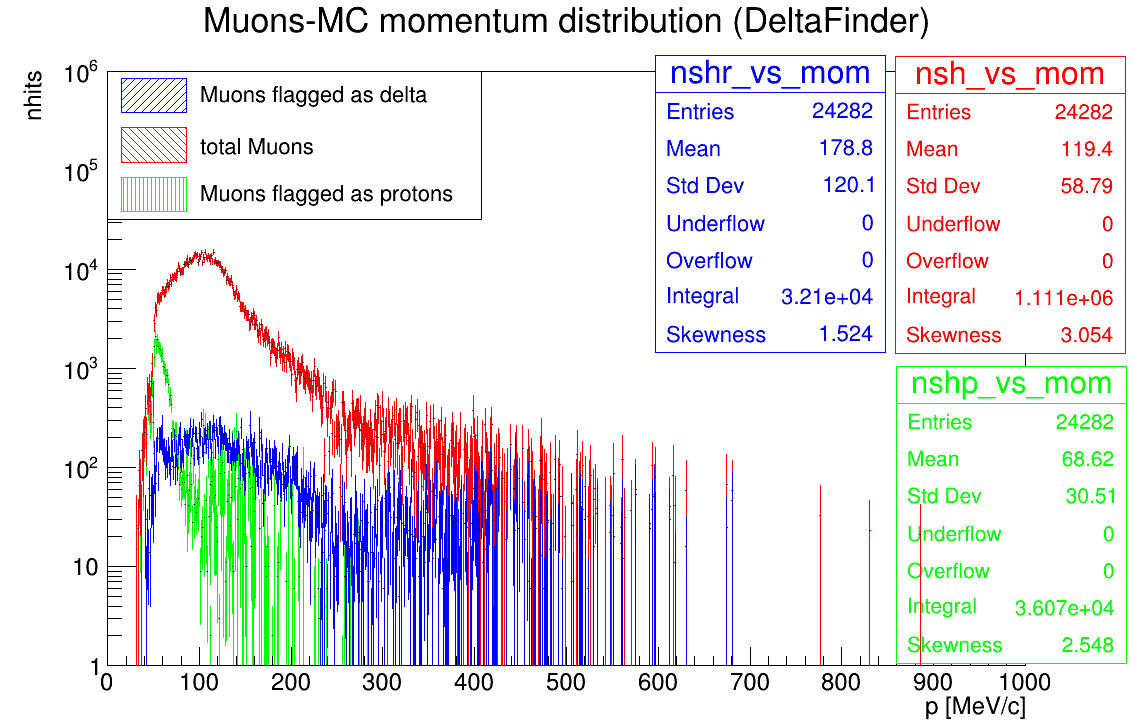
\includegraphics[width =0.8\textwidth]{figures/png/Screenshot_20240805_222923.png}
        \caption[The distribution of the total and flagged number of muon $ComboHit$s versus momentum.]{The 
        distribution of the total number of muon $ComboHit$s 
        (red) and those flagged as $\delta$s (blue) 
        and protons (green) versus the particle momentum ($PBAR0BB$ data sample). }
           \label{fig:0pbarbefore}
\end{figure}




Now let's move on to the performance analysis and comparison part.

Tables \ref{tab:2bbcele} and \ref{tab:1bbcele} show the hit-level 
comparison for the $CELE1BB$ and $CELE2BB$ data samples between the two algorithms.
\begin{center}
    \begin{table}[h!]
    \centering
    \renewcommand{\arraystretch}{1.}
    \begin{tabular}{| c | c | c | c | c | c |} 
    \hline
    &  $f_{p}$ FBH &  $f_{p}$ DF & $f_{e}$ FBH  & $f_{e}$ DF \\
    \hline
    e$^-$ ($p<$20 MeV/c)      & 2.5\% & 3.7\%   & 75.1\% & 72.7\%\\
    \hline
    e$^-$ (20$<p<$80 MeV/c)  & 1.1\% & 2.2\%   & 49.0\%& 29.9\%\\
    \hline
    e$^-$ (80$<p<$110 MeV/c)   & 0.2\% & 0.8\%  &  7.4\%& 4.3\%\\
    \hline
    $p$       &  &  83.6\%  &  & 2.2\%\\
    \hline
    e$^+$ ($p<$20 MeV/c)   & 0.6\%& 0.4\%    &   84.2\%& 87.9\%\\
    \hline
    \end{tabular}
    \caption[Electrons, 
    Positrons and Protons hit-level comparison.]{Electrons, 
    Positrons and Protons hit-level comparison ($CELE2BB$ data sample).}
    \end{table}\label{tab:2bbcele}
    \end{center}

    \begin{center}
    \begin{table}[h!]
    \centering
    \renewcommand{\arraystretch}{1.}
    \begin{tabular}{| c | c | c | c | c | c |} 
    \hline
    &  $f_{p}$ FBH &  $f_{p}$ DF & $f_{e}$ FBH  & $f_{e}$ DF \\
    \hline
    e$^-$ ($p<$20 MeV/c)      & 2.5\% & 2.5\%   & 75.9\% & 72.5\%\\
    \hline
    e$^-$ (20$<p<$80 MeV/c)  & 1.0\%& 1.0\%   & 50.0\%& 27.4\%\\
    \hline
    e$^-$ (80$<p<$110 MeV/c)   & 0.2\%& 0.3\%  &  5.7\%& 3.4\%\\
    \hline
    $p$       &              &         83.7\%           &  & 1.0\%\\
    \hline
    e$^+$ ($p<$20 MeV/c)   & 0.5\%    & 0.2\%    &   85.5\%& 88.5\%\\
    \hline
    \end{tabular}
    \caption[Electrons, Positrons and Protons hit-level comparison.]{Electrons, 
    Positrons and Protons hit-level comparison ($CELE1BB$ data sample).}
    \end{table}\label{tab:1bbcele}
    \end{center}
  
The fraction of electrons and positrons flagged as $\delta$-electrons 
differs due to the momentum distribution of these particles at low energies 
(Figure \ref{fig:efficiency}). These plots show the efficiency 
(i.e., the number of $\delta$-electron $ComboHit$s flagged as $\delta$s 
over the total number of $ComboHit$s for each particle type) as a function 
of particle momentum for positrons (red) and electrons (blue) using the 
$FlagBkgHits$ (left) or $DeltaFinder$ (right) algorithms. 

At low momentum values (less than 1-2 MeV/c), the efficiency 
is higher for positrons since the total number of $ComboHit$s 
with such low momentum is extremely small, as they are 
not affected by Compton scattering. The efficiency plot 
is in fact convoluted with the momentum distribution.

From both tables, it is also possible to notice that the positron 
efficiency for $FlagBkgHits$ is lower compared to $DeltaFinder$. 
This is because the MVA output is statistics-dependent. In this energy 
range, positrons have very few $ComboHit$s, as they are not 
affected by Compton scattering. Therefore, $FlagBkgHits$ performs 
better with higher statistics and is more efficient for $E < 2$ MeV/c. 
At the same time, $DeltaFinder$ works less effectively with electrons. 
This is due to the high number of $ComboHit$s at this energy range, 
while the number of $ComboHit$s flagged as $\delta$ remains constant 
at low energies, as Compton electrons have only one 
hit per station, making impossible to find the $seed$. 

For higher momentum values, both algorithms perform similarly, and 
the differences between positrons and electrons become negligible. 
The sum of the positron and electron efficiency (Tables \ref{tab:2bbcele} 
and \ref{tab:1bbcele}) for a given algorithm 
matches that of the other algorithm, indicating they have the same 
capability in rejecting $\delta$-electrons. 
For both the algorithms, the primary cause of failure 
in $\delta$ flagging arises from hits on straws that are 
parallel to each other, particularly those near the center of the tracker, 
where stereo reconstruction is not possible.

XXXXX PICCO A 50 MEV/c in fp

When discussing the differences between the two 
algorithms, particularly regarding CE flagging, 
there is a factor of 1.7 between the two $f_e$. 
The main difference is as follows: sometimes, CE hits 
can occur close in time and space to other $\delta$ hits. 
As a result, $FlagBkgHits$ flags them as $\delta$, since 
it does not attempt to locate corresponding hits in another station, 
while $DeltaFinder$ tries to connect $seed$s across the stations.


Concerning proton flagging, we could not compare the two 
algorithms since the $FlagBkgHits$, before creating $StereoHit$s, 
applies a preliminary selection cut on the energy deposited in 
the $StrawHit$s of 5 keV. Subsequently, the algorithm identifies 
protons as all particles with a deposited energy greater than 
4.5 keV. It was not possible to conduct a direct comparison, 
as $DeltaFinder$ does not apply a cut on the energy deposited in 
the $StrawHit$s, making the comparison unreliable and biased. 
The fraction of particles flagged as protons by $FlagBkgHits$ 
corresponds to the fraction of $ComboHit$s with a 
deposited energy higher than 4.5 keV and lower than 5 keV.

Therefore, we reported the fraction of protons 
flagged as protons by $DeltaFinder$.
This fraction underwent a reduction by a factor of 
1.1 after the applied cut (Table \ref{tab:1bbcelebefore}). 

From both Tables \ref{tab:2bbcele} and \ref{tab:1bbcele}, 
we can observe that the fraction of electrons misidentified 
as protons decreases with increasing momentum. This is because 
lower-energy electrons tend to have a higher deposited energy 
compared to others. This occurs because energy loss is dependent 
on particle energy, which increases as the energy decreases, 
leading to the misidentification of these electrons. Positrons, 
however, are not affected by this misidentification, as they 
are unaffected by Compton scattering and are not abundant in this energy range.

The results show the same conclusions for both the 1BB and 2BB data samples.

    \begin{figure}[!h]
        \centering
        \begin{subfigure}[t]{0.5\textwidth}
            \centering
            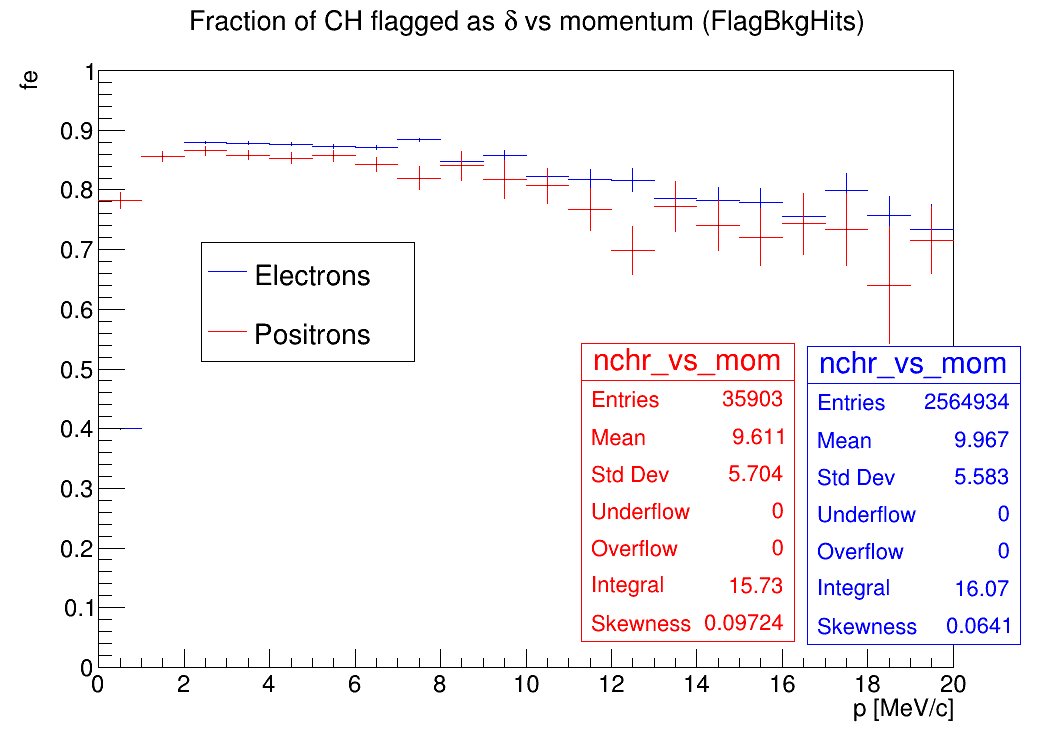
\includegraphics[width=1.\textwidth]{figures/png/Screenshot_20240818_155835.png}
            \caption{}
        \end{subfigure}%
        ~ 
        \begin{subfigure}[t]{0.5\textwidth}
            \centering
            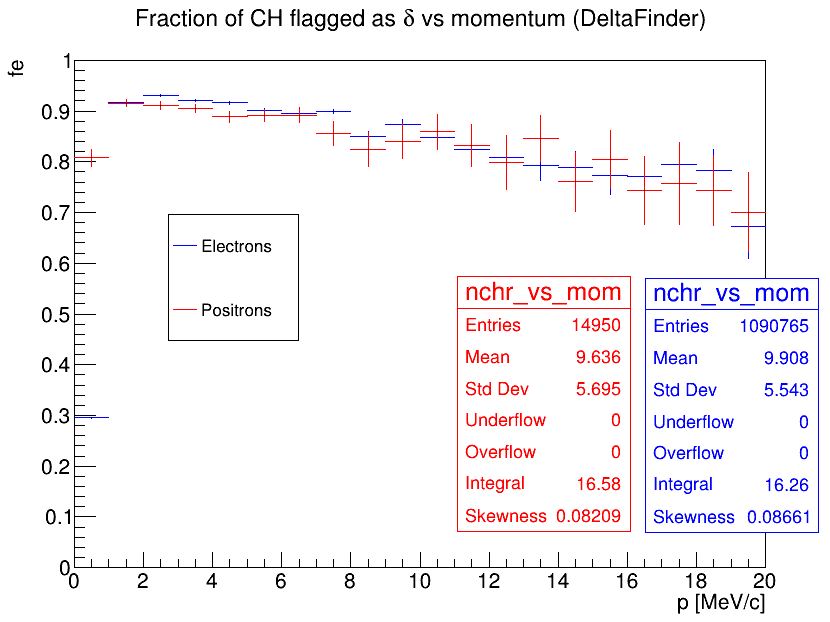
\includegraphics[width=0.95\textwidth]{figures/png/Screenshot_20240813_203916.png}
            \caption{}
        \end{subfigure}
        \caption[The efficiency of electrons and positrons versus 
        particle momentum in the low-momentum range.]{The efficiency of electrons (blue) and positrons (red) versus 
        particle momentum in the low-momentum range. The left plot shows the 
        results for $FlagBkgHits$, while the right plot shows those for $DeltaFinder$.
        }
        \label{fig:efficiency}
      \end{figure} 

      Looking at the results for $\mu$ and $\pi$ (Table \ref{tab:0bbpbar}), 
      we observe an approximate factor of 4 difference between the two algorithms 
      in muon delta flagging, and about a factor of 3.3 for pions. This occurs 
      because muons and pions often produce more than one hit in a single station, 
      but the $DeltaFinder$ algorithm is able to distinguish these hits, aided by 
      its ability to recognize straight lines in the $r-z$ plane, whereas 
      $FlagBkgHits$ cannot. Moreover, the problem with having a supervised 
      training method that distinguishes one type of particle from another 
      is that it can become confused when another particle, such as a cosmic 
      muon background event or tracks from $p\bar{p}$ annihilation, appears. 
      
      On average, pions from $p\bar{p}$ collisions have higher 
      momenta than muons, leading to a higher false positive rate. In fact, 
      there are more low-energy particles in the case of muons, making them 
      less likely to be correctly distinguished compared to pions. Furthermore, 
      the false positive rate ($f_p$) decreases as the momentum increases for pions, 
      according to the Bethe-Bloch formula.

    \begin{center}
        \begin{table}[h!]
        \centering
        \renewcommand{\arraystretch}{1.}
        \begin{tabular}{| c | c | c | c | c|} 
        \hline
        &$f_{p}$ FBH  &  $f_{p}$ DF &  $f_{e}$ FBH & $f_{e}$ DF\\
        \hline
        $\mu$ & 0.8\% &  2.7\%  & 13.0\% & 3.2\%\\
        \hline
        $\pi$ & 0.2\%& 0.4\% & 23.8\%& 7.3\%\\
        \hline
        \end{tabular}
        \caption[Muon and Pion hit-level comparison.]{Muon and Pion 
        hit-level comparison ($PBAR0BB$ data sample).}
        \end{table}\label{tab:0bbpbar}
        \end{center}


\subsection{Track-level comparison}
At this point the unflagged hits were sent to the pattern recognition and the reconstruction was performed. 
Table \ref{tab:recoeffcele} reports the reconstruction efficiency, defined as the 
number of reconstructed track over the total number of events, and the efficiency 
after selecting the true CE tracks (both 2BB and 1BB), while Table \ref{tab:recoeffpbar} 
shows the reconstruction efficiency and the efficiency after applying selection cuts for the $p\bar{p}$ analysis. 
Table \ref{tab:recoeffcele} indicates that there is a difference of 
approximately 20\% between the number of reconstructed tracks using 
$FlagBkgHits$ and $DeltaFinder$. However, when selecting tracks that 
correspond to CEs, the efficiency is almost identical.

\begin{center}
    \begin{table}[h!]
    \centering
    \renewcommand{\arraystretch}{1.}
    \begin{tabular}{| c | c | c | c | c |} 
    \hline
    & FBH,2BB & DF,2BB & FBH,1BB & DF,1BB  \\
    \hline
    tracks reconstruction efficiency & 52.8\% &  42.9\% & 47.8\% & 41.3\%\\
    \hline
    CE reconstruction efficiency & 30.9\% & 31.2\% & 32.0\% & 32.2\%\\
    \hline
    \end{tabular}
    \caption{}
    \end{table}\label{tab:recoeffcele}
\end{center}

This table can be understood by examining Figure \ref{fig:highlevel1}, 
which shows the momentum distribution of reconstructed tracks. In the 
case of $FlagBkgHits$ (blue), protons are not correctly flagged, so 
they are sent to pattern recognition and then reconstructed. On the 
other hand, $DeltaFinder$ (red) is able to flag and count proton hits, 
preventing them from being sent to pattern recognition. When selecting 
Monte Carlo truth, meaning all particles that are actually CE, the 
distribution appears as in Figure \ref{fig:highlevel2}. The number 
of reconstructed CEs is nearly the same. 
Table \ref{tab:recoeffcele} reveals a difference in the 
reconstructed track efficiency for $FlagBkgHits$ 
between 2BB and 1BB, which depends on the number of protons reconstructed. 
In fact, in 2BB, the number of proton reconstructed tracks is higher than in 1BB case. 
For the rest, the results are similar for both 1BB and 2BB.


\begin{figure}[!h]
    \centering
    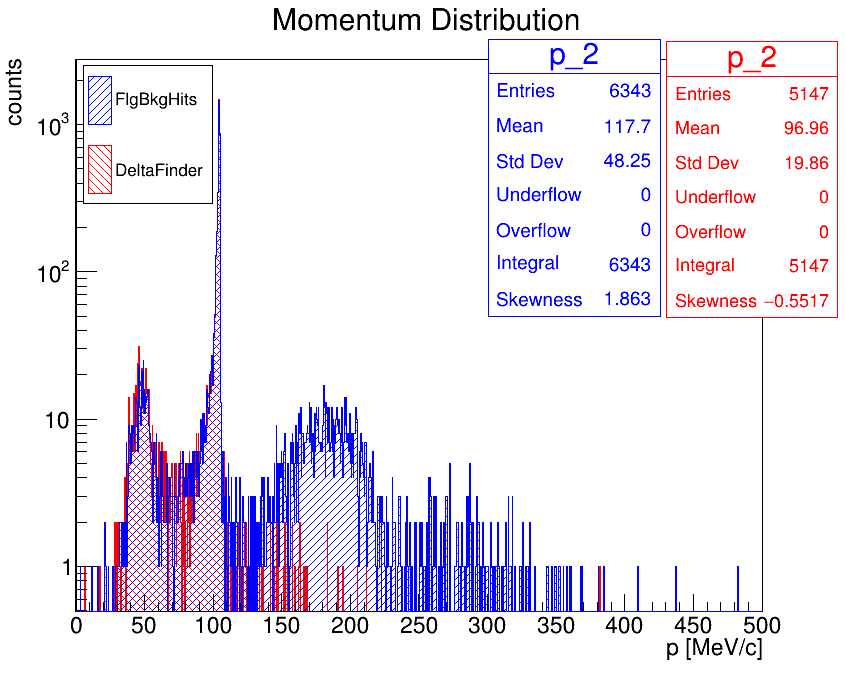
\includegraphics[width =0.8\textwidth]{figures/png/Screenshot_20240813_171301.png}
    \caption[]{}
    \label{fig:highlevel1}
\end{figure}
\begin{figure}[!h]
    \centering
    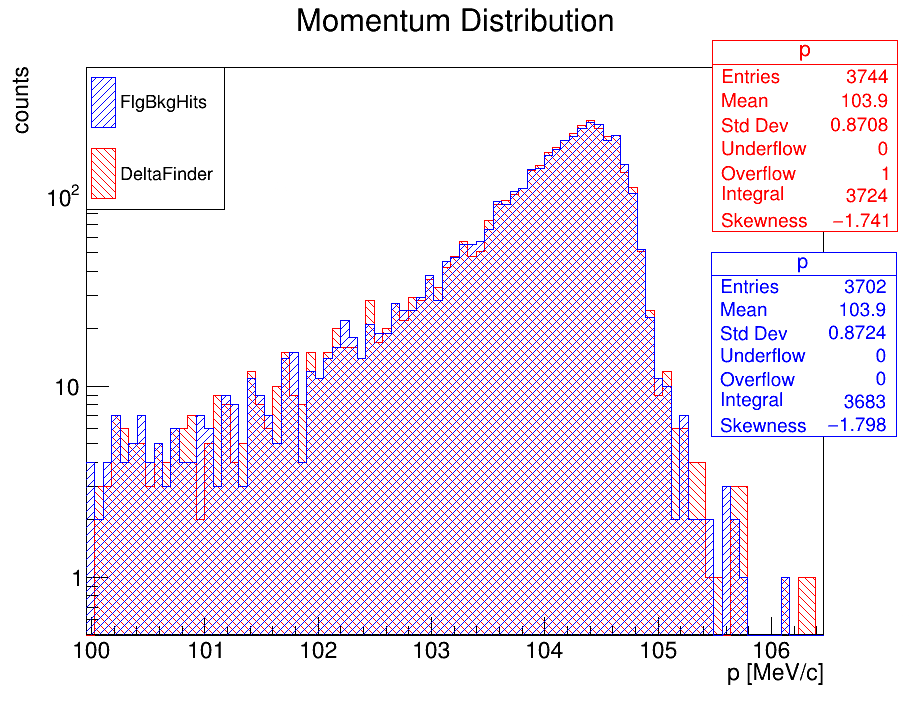
\includegraphics[width =0.8\textwidth]{figures/png/Screenshot_20240813_171330.png}
    \caption[]{}
    \label{fig:highlevel2}
\end{figure}
We tried to look at those events where at least one track 
was reconstructed in the case of one hit flagger and no 
tracks reconstructed in the case the other one.
There is a well defined class of events where the 
effects of hit flaggers get washed out in the 
reconstruction by the time clustering algorithm.
Figure \ref{fig:TZCluster1} ($FlagBkgHits$) and \ref{fig:TZCluster2} ($DeltaFinder$) show 
an the same example event for the two algorithms, in particular the $time$ 
versus $z$ coordinate (the one along the tracker).
The violet squares contain particles related to the same $TimeCluster$. 
This is searched from hits that fit along a linear
line in time versus z space. These hits are first combined in some time-z window to create $chunks$ (at present
the time window is 20 ns and z-window of 5 planes). A window is considered to be a $chunk$ if
more than 3 ComboHits are within it. Every possible pair of chunks that are within some time of each other are tested together. The
pair that yields the smallest $\chi^2/ndof$ when the hits are fit to a linear line are permanently
combined. This is repeated until no new combination yields a $\chi^2/ndof$ below some threshold. If
the chunk exceeds some minimum number of straw hits it is saved as a cluster. 
In the two plots CE hits are the big red dots, delta elctrons the small brown ones and protons are the big blue dots. 
$TimeCluster$s have different $z$ value, since the particles that are grouped together, can be at different $z$ 
The two plots show that in the first case the hits are all grouped in the same 
cluster (green) and in the second one (green and orange) CE hits are grouped in two different $TimeCluster$s. 
An example is described in the following lines. 
In the case of $DeltaFinder$, hits from the same 
particle are divided in two different time clusters, but for 
$FlagBkgHits$ the not flagged hits are used by the time clusterer to $connect$ 
particle hits that are used in the reconstruction. 
That is why the track is reconstructed in this case. 
Improving the cluster finder and the pattern recognition 
could increase the track reconstruction performance.
\begin{figure}[!h]
    \centering
    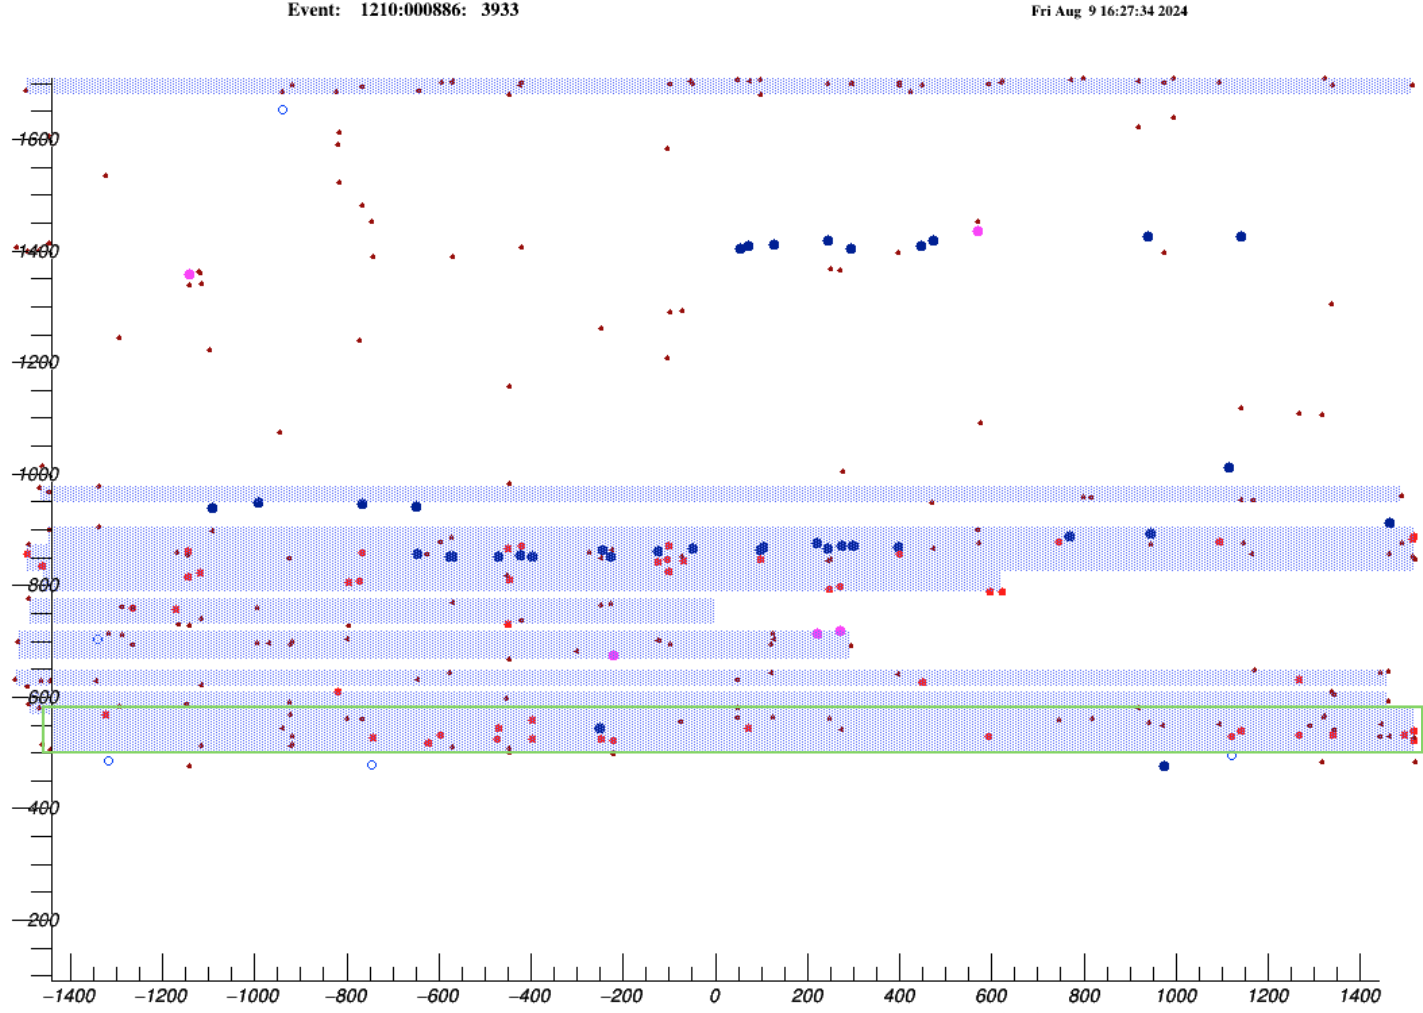
\includegraphics[width =0.8\textwidth]{figures/png/Screenshot_20240819_153229.png}
    \caption[]{}
    \label{fig:TZCluster1}
\end{figure}
\begin{figure}[!h]
    \centering
    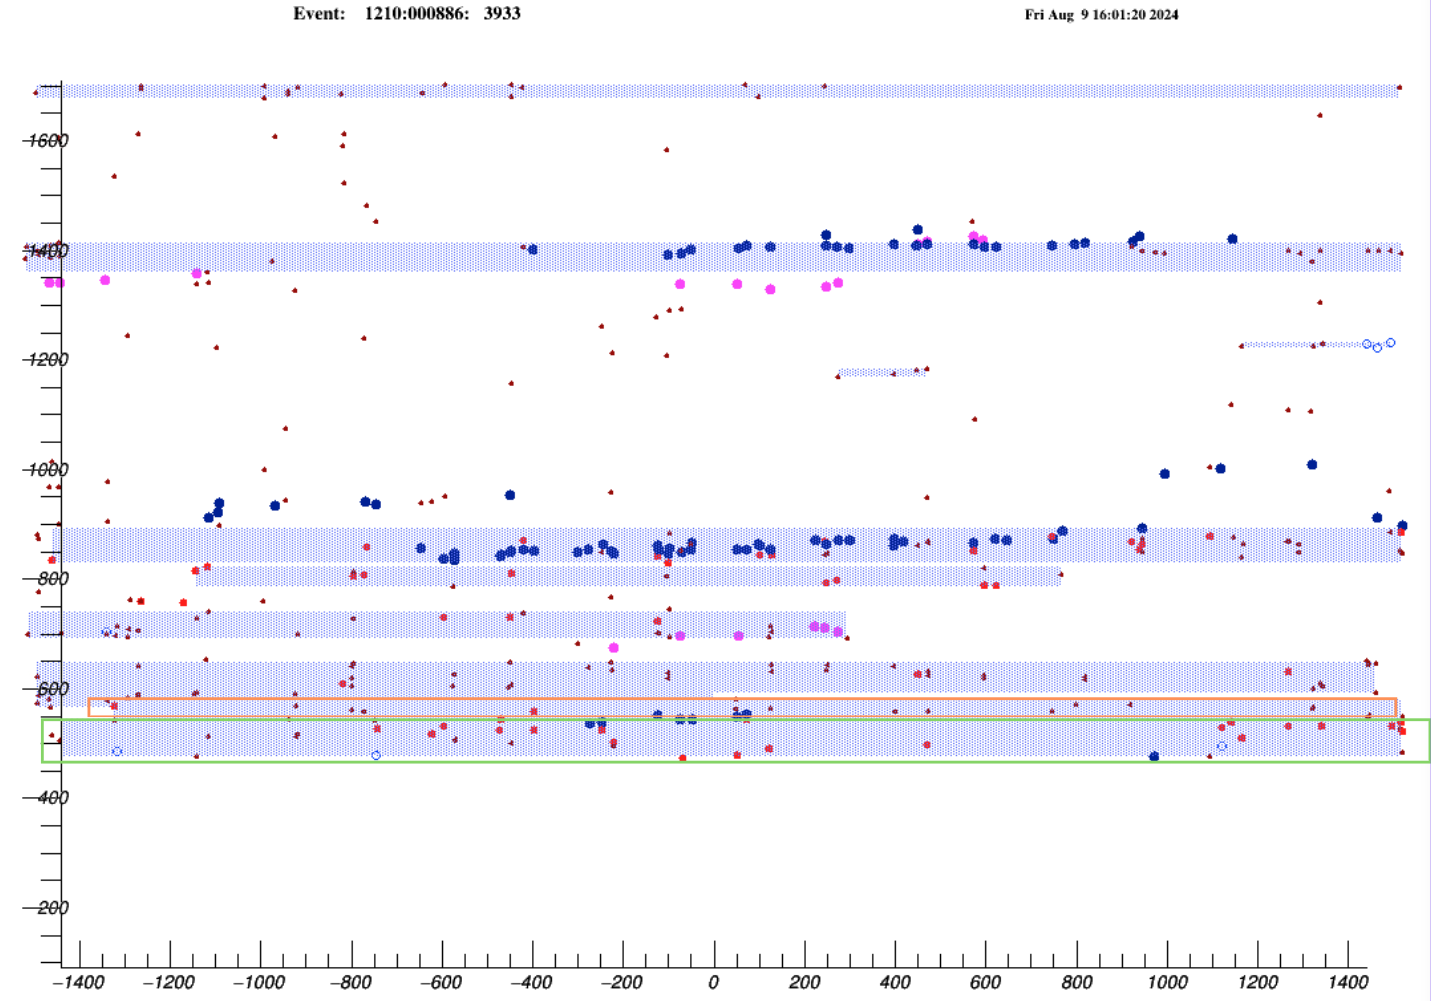
\includegraphics[width =0.8\textwidth]{figures/png/Screenshot_20240819_153730.png}
    \caption[]{}
    \label{fig:TZCluster2}
\end{figure}
Delta finder has an advantage for 2 track reconstructed. This comes from 
the fact that a larger number of hits are left with $DeltaFinder$.
A particle trajectory can be considered a viable candidate for 
reconstruction if it makes at least 20 hits in the tracker and if the 
reconstructed $\chi^2/ndof\leq 3$.
Here are reported two different momentum selection cuts. 
For particle coming from the stopping target, 
you dont have enough hits to reconstruct particles with 
momentum below 80 MeV/c, that is why we selected the first momentum cut. 
Moving to 90 MeV/c is to eliminate completely the DIO.
Requiring the DIO electron momentum to
be above 90 MeV/c gives an estimate of about $10^{-2}$
events with two DIO electrons for Run I. Assuming a track reconstruction
efficiency of $\sim$0.1, we reconstruct about $10^{-4}$ events with
two DIO electron tracks. Further, assuming a uniform distribution in time, the number of events with two DIO electrons
within a time window of 100 ns is $\sim10^{-5}$.
\begin{center}
        \begin{table}[h!]
        \centering
        \renewcommand{\arraystretch}{1.}
        \begin{tabular}{| c | c | c |} 
        \hline
        &  FBH & DF \\
        \hline
        tracks reconstruction efficiency ($Ntracks \geq 2$) &  3.8\% & 4.6\%\\
        \hline
        reconstruction efficiency after selection (p$>$80 MeV/c) & 3.0\% & 3.8\%\\
        \hline
        reconstruction efficiency after selection (p$>$90 MeV/c) & 2.7\% & 3.2\%\\
        \hline
        \end{tabular}
        \caption{}
        \end{table}\label{tab:recoeffpbar}
\end{center}


    
    Cose da capire e fare: 
    1) perche il picco su 50MeV/c sulla fp degli elettroni
    4) devo far levare anche FBH fp?

6)high level bench mark
7) tzcluster
9)timing
8)fare rif a piu numeri
cerca di capire 1hit/track
1hit/track*7701tracks=7701 hits che rappresenterebbe 14150-8168 combohits
\section{Conclusions}
e'basato sul monte carlo. training difficile. se e' sviluppato per 
riconoscere bene A e B, quando arriva C va in confusione. lavora male quando la statistica e'bassa. 
non distingue i protoni.
